\documentclass[12pt]{article}
\usepackage{amssymb}
\usepackage{graphicx}
\usepackage{setspace}
\usepackage{geometry}
\usepackage{gensymb}
%\usepackage{epsfig}
\linespread{1.9}

\geometry{
  body={5in, 8.5in},
left=1.25in,
right=1.25in,
  top=1.5in
}


\begin{document}

\title{Physics 715 Term Project:  Numerical Tools \& Aerodynamic Engineering}
\author{Ben Keller}
\maketitle
\newpage

\section{Introduction}
A most remarkable application of the principles of fluid mechanics is that of
heavier than air flight.  Through the application of theory developed by 
Prandtl, Bernoulli, and others, humankind has been constructing aircraft for 
over a century.  Aerospace engineering has become a major part of Western 
industry, accounting for 1.6\% of Canada's GDP in 2008, with a total industry
revenue of over \$20 billion in that same year[1].  The innovation that fuels
this engine of wealth creation is driven by the use of fluid mechanics in 
designing better airfoils and aerodynamic structures.  This process is now 
almost exclusively done using numerical simulations of the Navier-Stokes
Equations with the boundary conditions for the designs being tested.  These 
tools allow rapid turnaround between computer-aided design (CAD) of products
to numerical simulations of their performance, and further revision of the
designs.\par

In this project, I hope to show an outline of the work that goes into designing
a typical component in which hydrodynamic simulations are an important part of
the design process.  These tools are used beyond the aerospace field, and are 
important in the design of products ranging from sports cars to ship propellers
and plumbing.  I will begin by posing a simple design problem: Can a 
cylindrically-symmetrical airfoil be designed and used to focus the airflow
from a fan and improve its performance?  I will design 3 test cases, and simulate
them using a hydrodynamic code with 3D CAD models I will build for each case. 
From this simulation, I will compare the quantitative performance of each case,
and determine the best design.

\section{A Simple Design Problem}
One of the most elementary cases examined in fluid mechanics is that of flow 
over an airfoil.  As the airfoil produces vorticity from the formation of a
viscous boundary layer on along it's surface (a result of the Kutta condition),
it experiences a lifting force proportional to the circulation $\Gamma$ about
its surface, and the flow velocity $u$ relative to the airfoil:
$$F_L = \rho u \Gamma$$
Besides the obvious application of lifting wings on aircraft, airfoils are 
frequently used to duct fans and wind turbines to increase the performance
therein by utilizing the same vorticity effect to push more air across the fan
or wind turbine blades.  I would like to examine this by designing an airfoil
for use around a simple computer cooling fan.  I will examine the flow 
properties of this airfoil in a $10\times10\times10cm$ square duct, similar in
size to a typical ATX computer power supply.

\section{Three Airfoil Designs}
The airfoils I tested were 3 simple designs: a simple hollow cylinder, a $4cm$ long airfoil, and a $2cm$ long airfoil.  The shapes of the
airfoils are discussed in section below.
The fan I will design the airfoil for is a $7cm^2$ square 12V DC fan, rated to 
pump air at a rate of 70 cfm (cubic feet per minute).  This results in a fluid
velocity of roughly $6.7m/s$.  As the airfoil will have a diameter of $7cm$, 
this results in a Reynolds number (in air, at 25\degree C, the kinematic viscosity is 
$\approx1.56*10^{-5} m^2/s$) of:
$$R_e = \frac{UL}{\nu} = \frac{6.7*0.07}{1.56*10^{-5}} = 3.0*10^4$$
This large Reynolds number implies that turbulence may become an important for
accurately modelling this situation.

I chose two NACA airfoils for my experiment, NACA5440 with a length of $2cm$
and NACA5420 with a length of $4cm$ .  This pair was chosen so that the airfoil
with twice the length (NACA5420) would have the same aperture diameter (since it has half the thickness of NACA5440).  The rectangular airfoil was simply a $4
\times 0.5cm$ box.

\begin{figure}[H]
\centering
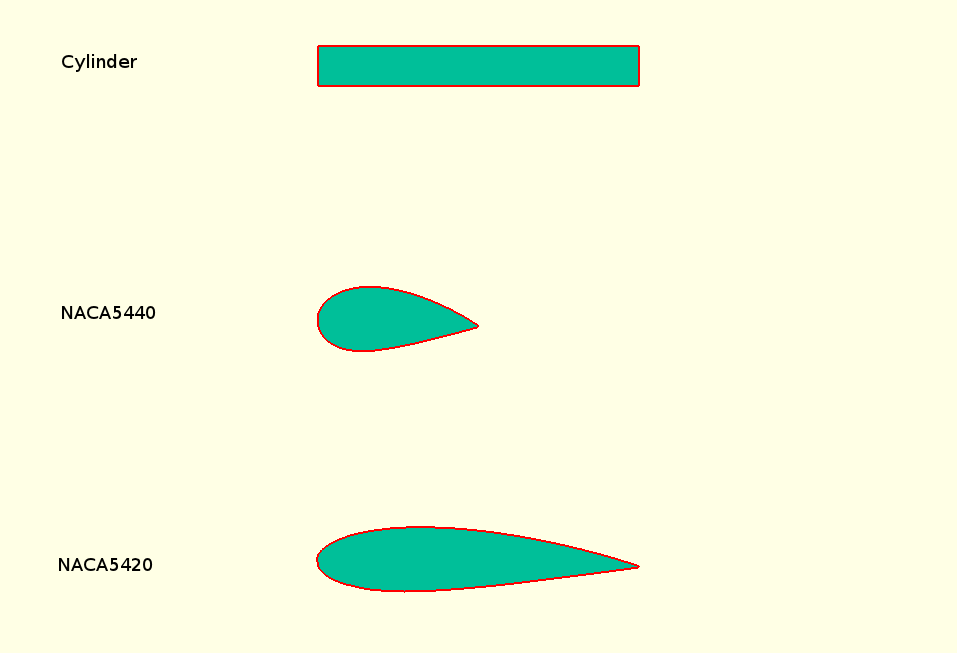
\includegraphics[width=6in]{../images/airfoils.png}
\caption{Cross-sections of my 3 airfoils}
\end{figure}

\subsection{NACA Parametric Airfoils}
The two lifting airfoils I will test are based on the National Advisory
Committee for Aeronautics (NACA)'s four digit series of parametric airfoils.
Ironically, these airfoils were designed and tested in 1933, long before 
digital computers became widely available.  The NACA airfoils are described
by a series of parametric equations of three variables.  The three variables,
$m$, $p$, and $t$ describe the fractional camber, the location of the
maximum camber in the x-axis, and and the fractional maximum thickness.  The
camber of the airfoil is a measure of the asymmetry between the upper and lower
surfaces, and is measured as the fraction of the distance of the maximum on the
curve of mean thickness from the x-axis over total length of the airfoil.  The
fractional maximum thickness is simply a ratio of the maximum thickness in the
y-axis over the length $l$ of the airfoil.  Expressed as percentages, the first
digit of $m$ and $p$, and the first two digits of $t$ define the airfoil 
NACA MPTT (ie, NACA 1234 has a maximum camber of 10\%, located at 20\% of its
total length, and has a thickness 34\% of its length).  The equations that
define the upper $(x_U, y_U)$  and lower $(x_L, y_L)$ surfaces of these 
airfoils are as follows:
$$x_U = x - y_t\sin\theta, \quad y_U = y_c+y_t\cos\theta$$
$$x_L = x + y_t\sin\theta, \quad y_L = y_c-y_t\cos\theta$$
$$\theta = \tan^{-1}(\frac{dy_c}{dx})$$
$$y_t = \frac{t}{0.2}l[0.2969\sqrt{\frac{x}{l}}-0.1260(\frac{x}{l})-
0.3516(\frac{x}{l})^2+0.2843(\frac{x}{l})^3-0.1015(\frac{x}{l})^4]$$
\[y_c = \left\{\begin{array}{l l}
    m\frac{x}{p^2}(2p-\frac{x}{l}) & \quad 0 \le x \le pl \\
    m\frac{l-x}{(1-p)^2}(1+\frac{x}{l}-2p) & \quad pl \le x \le l\\
  \end{array} \right.
\]

\section{Numerical Methods}
As the reader may be aware, the Navier-Stokes Equations are a system of 
nonlinear partial differential equations that describe the flow of viscous
fluid.  The equations determine the evolution of the velocity field in the
fluid $\mathbf{v}$ in relation to the body forces $\mathbf{F}$, the stress 
on the fluid $\mathbb{T}$, the density $\rho$, and the pressure $P$.  The
equations are defined as follows:
$$\rho\frac{D\mathbf{v}}{Dt} = -\nabla P +\nabla\cdot\mathbb{T}+\mathbf{F}$$
Finding solutions to these equations beyond simple cases,
as with finding solutions for any system of nonlinear PDEs, usually comes to
finding numerical solutions.

\subsection{Domain Decomposition \& Meshing}
The first step in testing my airfoils was to model them in a Computer Aided
Design program.  I used OpenSCAD to generate the 2D slices of the airfoils
using the parametric equations, and then ``extruded'' them in a $3.5cm$ radius
circle about the z-axis.  This extrusion process is equivalent to defining
the $x$ and $y$ coordinates of the NACA equations to be the $z$ and $r$ 
coordinates of a cylindrical coordinate frame, and integrating the equations 
about the $\theta$ axis.  An example of the resulting 3D surface is shown in
figure NUM.

\begin{figure}[H]
\centering
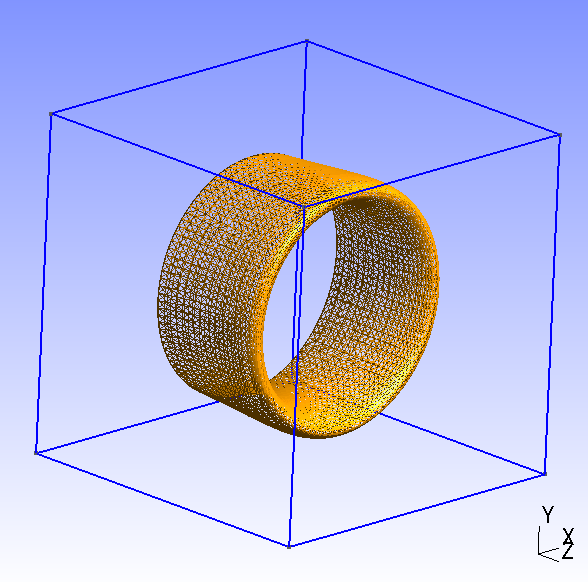
\includegraphics[width=6in]{../images/NACA5420.png}
\caption{NACA5420 airfoil extruded in 3D}
\end{figure}

Once the airfoil has been designed using OpenSCAD, it can be exported as a 
Standard Tessellation Language (STL) file.  This file contains a series of
vertices and unit normals describing a triangular tessellation of the airfoil
surface.  I then wrote a script for the finite element mesh generator gmsh that
defined the volume of the simulation, with the airfoil STL centred in a 
$10\times 10\times 10 cm$ box.  Gmsh then automatically decomposed the volume
of the box into a tetrahedral mesh.  This meshing is essential for the Finite
Volume method, which will be discussed in the next section.
An example of the resulting mesh is shown in figure NUM.


\begin{figure}[H]
\centering
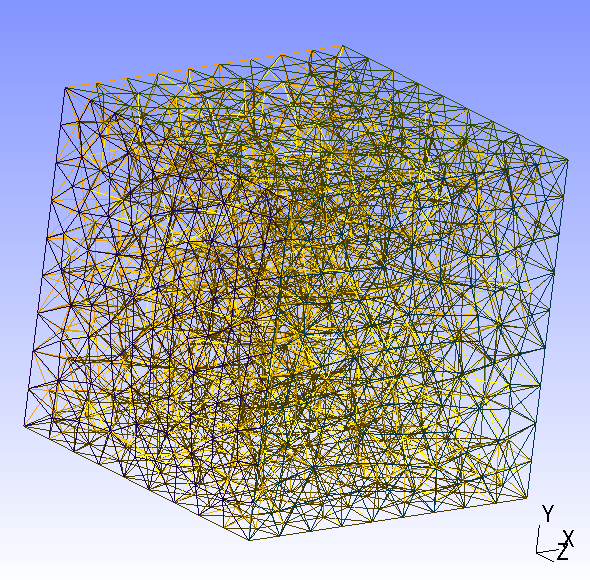
\includegraphics[width=6in]{../images/mesh.png}
\caption{Domain decomposition mesh generated by gmsh}
\end{figure}

\subsection{Code\_Saturne}
The tool I used for solving the Navier-Stokes equations in the case
of flow around my airfoils was a 
suite of software tools written by the French utility corporation 
\'{E}lectricit\'{e} de France (EDF), Code\_Saturne.  
\subsubsection{Discretization \& Numerical Solver}
Naturally, the first step one would expect in trying to solve a system of
equations such as the Navier-Stokes would be to discretize the problem: to split
the time and space components into finite elements.  The splitting of the fluid
volume into cells makes this solution one of a class of solutions known as 
Finite Volume Models.  The general transport equation that Code\_Saturne solves
is for the transport of quantity $f$, with sources $S$, density $\rho$, 
kinetic energy $K$, and fluid velocity $\mathbf{u}$, is:
$$\rho\frac{\partial f}{\partial t} + \nabla\cdot((\rho\mathbf{u})f) - 
\nabla\cdot (K\nabla f) = Sf+\nabla\cdot(\rho\mathbf{u})f$$
By solving this equation, the transport of any quantity can be determined.

Code\_Saturne offers a number of time discretization methods, all from the 
family of linear multistep methods.  I used the simplest, 1st order method, 
where a quantity $\Phi$ is calculated at timestep $n+1$ using the value at 
timestep $n$ and $n-1$:
$$\Phi^{n+1} = 2\Phi^n-\Phi^{n-1}$$
The discrete form of the general transport equation, for timesteps of 
$\Delta t$:, is:
$$\frac{\rho}{\Delta t}(f^{n+1}-f^n)+\nabla\cdot((\rho\mathbf{u})(f^{n+1})
-\nabla\cdot(K\nabla f^{n+1})=[Sf]^{n+1} + \nabla\cdot(\rho\mathbf{u})f^{n+1}$$
This allows the incremental calculation of quantities at timestep $n+1$ using
the properties of the flow and the quantity at timestep $n$.

The volume discretization simply uses the non-spatially varying elements to be
averaged over the volume of the cell.  Divergences are simple to calculate in
this discrete form using Green's Theorem:
$$\nabla\cdot \Phi = \displaystyle\sum\limits_{i,j \in Neighbour(i)}\Phi_{ij}
S_{ij}$$
In other words, the divergence of quantity $\Phi$ is simply the sum over all
cells $i$ with faces intersecting cells $j$, with surface area $S_{ij}$ and
$\Phi_{ij}$ on the interface between them.  By iterating the general transport
equation over every cell face, and matching the boundary conditions on the 
edges of every intersecting cell, a continuous volume evolving over a continuous
period of time can be broken down into a discretized volume of finite cells
evolving over a finite number of timesteps in an iterative process.  A more 
thorough examination of the numerical methods used in Code\_Saturne and other
Navier-Stokes solvers is beyond the scope of this paper.  For a full treatment
of Code\_Saturne's architecture, see [3] and [5].
\subsection{Usage}
Code\_Saturne read the mesh I generated earlier, using the mesh elements as the
3D domains in the finite element method.  I gave the tool fluid properties
(density, temperature, viscosity) of air at 25\degree C, and defined the 
boundary conditions such that the cube faces around the airfoil were solid 
walls, but the face in front of the airfoil was an inlet, pumping air in at
$6.7m/s$, and the face behind the airfoil was an outlet, allowing air to escape
without piling up.  I gave the air in the box an initial velocity of $6.7m/s$
in the $-z$ direction, so that there wasn't a discontinuity in flow velocity
at the inlet.  I used Code\_Saturne's steady, single phase flow solver, along
with the $k-\epsilon$ turbulence model.  While by definition turbulent flow 
is unsteady, the bulk flow in this case is steady, and so this solver can be
used.  I ran the simulation for a total of 1 second, with timesteps calculated
automatically.
I ran 4 cases with Code\_Saturne: an empty box, and 1 for each of my 3 airfoils.
Code\_Saturne produced a file that could be read using ParaView to examine
various physical properties in 3D.

\subsubsection{Turbulence Modelling}
The turbulence model I used for this project was the $k-\epsilon$ model.  This
technique works by solving for the transport of two scalar values: the 
turbulent kinetic energy $k$ and the turbulent dissipation (in other words,
the turbulence scale) $\epsilon$.  This model depends only on the Reynolds 
stress tensor $\mathbb{R}$, fluid density $\rho$, and dynamic viscosity $\mu$.
The equations describing this model are shown below, for the case of an
incompressible flow without sources or sinks:
$$k = \frac{1}{2}R_{ij}$$
$$\mathcal{P} = -\rho R_{ij}\frac{\partial u_i}{\partial x_j}$$
$$\rho\frac{Dk}{Dt} = (\mu+0.009\frac{k^2}{\epsilon}\nabla k)+\mathcal{P} -
\rho\epsilon$$
$$\rho\frac{D\epsilon}{Dt} = (\mu+0.007\frac{k^2}{\epsilon}\nabla\epsilon) +
1.44\frac{\epsilon}{k}\mathcal{P} - 1.92\rho\frac{\epsilon^2}{k}$$
As the reader may deduce, the first term of the two transport equations act
as a turbulent viscosity term that feeds back to the full Navier-Stokes 
Equations:
$$\mu_t = 0.009\rho\frac{k^2}{\epsilon}$$
The derivation of this model is beyond the scope of this project, and can be 
found in [5].  

\section{Results \& Analysis}
I compared the resulting simulation using data generated using the ParaView 
utility.  I used this tool to obtain a 2 dimensional slice of the simulated
volume, normal to the z-axis, and $1cm$ from the exit of the airfoil.  This 
slice contained measurements at points on the surface (based on the number of 
intersecting mesh cells) for pressure, velocity, and energy stored in 
turbulence. Figure NUM shows streamlines plotted around the NACA5420 airfoil
using ParaView.  Figure NUM shows one of the slices I used to get data points.

\begin{figure}[H]
\centering
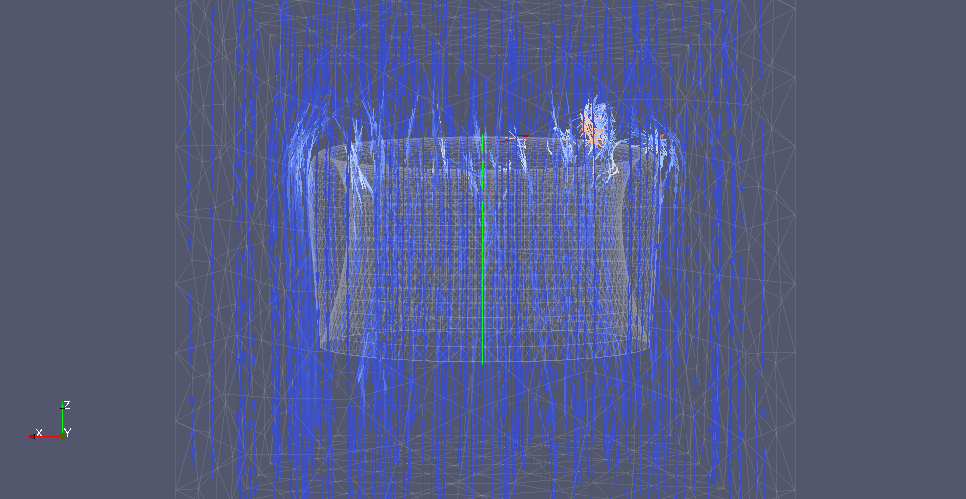
\includegraphics[width=6in]{../images/NACA5420_streamlines.png}
\caption{Streamlines flowing across NACA5420 airfoil, colored by turbulent
kinetic energy}
\end{figure}

\begin{figure}[H]
\centering
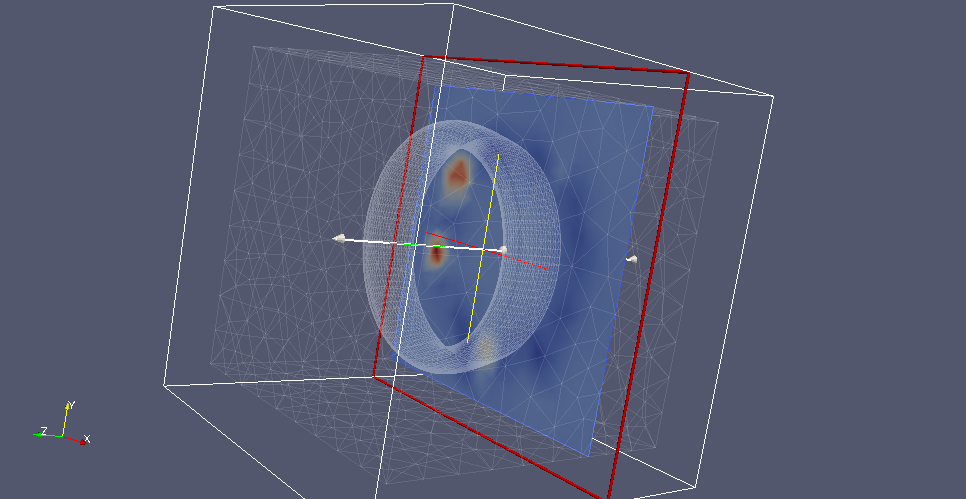
\includegraphics[width=6in]{../images/slice_generation.png}
\caption{Slice through flow $1cm$ behind NACA5440 airfoil, colored by velocity}
\end{figure}

I used python, along with the Numpy numerical module and matplotlib plotting
utility to produce plots of the velocity through the slice, the turbulent energy, and an approximation of vorticity magnitude $\bar\omega$
calculated using the velocity component parallel to the plane $v_{||}$:
$$\bar\omega = rv_{||}$$


As figure NUM shows, NACA5440 had the highest total airflow, with a mean flow
velocity of $6.87m/s$.  However, the high spread suggests this is due to 
turbulence, and not a bulk flow.  The low spread on the NACA5440 airfoil 
is a desirable trait for a cooling fan, as you won't find pockets of hot
and cool forming because of inconsistent flow rate.  Figure NUM confirms my
suspicion about turbulence in NACA5440, with a much higher turbulent energy loss
than even the empty box.  NACA5420 also has the nice property of very laminar
flow, with vorticity close to zero across the entire flow surface, as shown in
figure NUM.  A table of average and RMS velocities through the surface is shown
in the table below.\\

\begin{figure}[H]
\centering
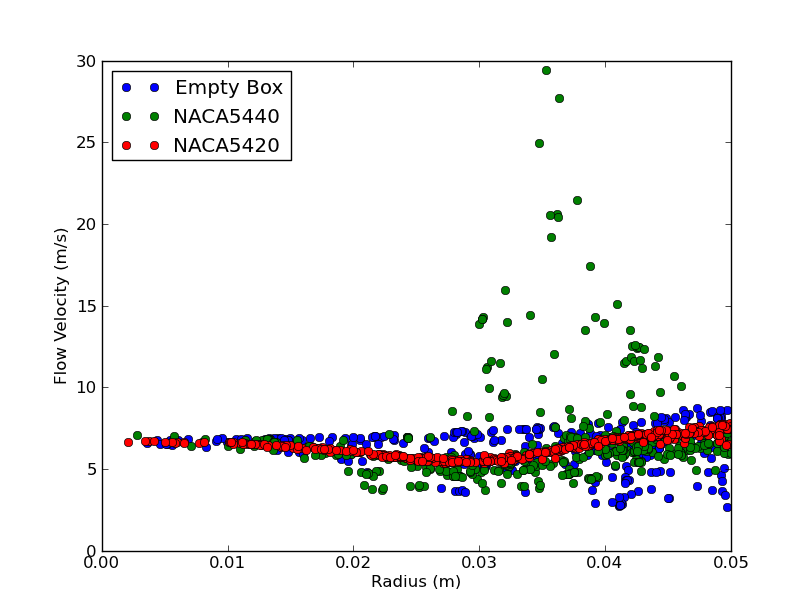
\includegraphics[width=5in, clip=true, trim=0in 0in 0.5in 0.5in]{../images/velocity_profile.png}
\caption{Z component velocity profile}
\end{figure}

\begin{figure}[H]
\centering
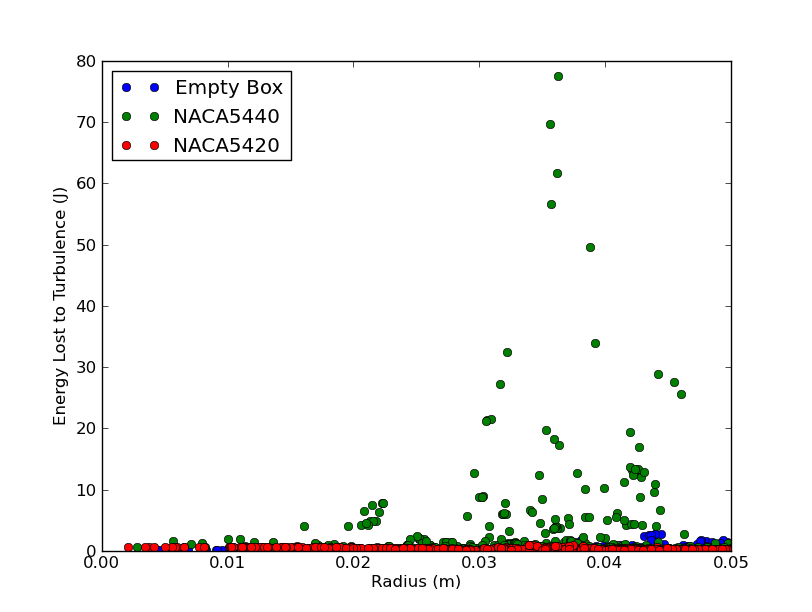
\includegraphics[width=5in, clip=true, trim=0in 0in 0.5in 0.5in]{../images/turb_profile.png}
\caption{Turbulent energy profile}
\end{figure}

\begin{figure}[H]
\centering
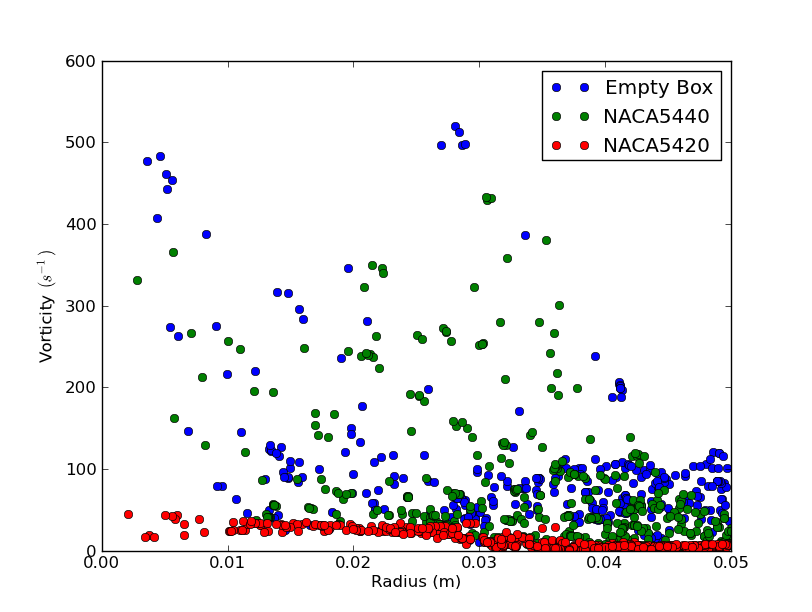
\includegraphics[width=5in, clip=true, trim=0in 0in 0.5in 0.5in]{../images/vorticity_profile.png}
\caption{Z normal vorticity profile}
\end{figure}

\begin{tabular}{| l | l | l |}
\hline
Case & Mean Velocity (m/s) & RMS Velocity (m/s) \\
\hline
Empty Box & 6.36 & 1.3 \\
NACA5440 & 6.87 & 3.2 \\
NACA5420 & 6.43 & 0.66 \\
\hline
\end{tabular}

\subsection{Pitfalls}
The biggest issue I came across during this project was the clearly incorrect 
turbulent velocities generated in the simple cylinder case.  As figure NUM 
shows, the velocity at a number of points on the test surface were actually
greater than $c$!  This I believe is a result of numerical divergence in the
turbulence $k-\epsilon$ model, and the sharp edges of the cylinder. Figure NUM
shows that the turbulent energy within the flow is absurdly high, peaking at
$10^{18}J$.

\begin{figure}[H]
\centering
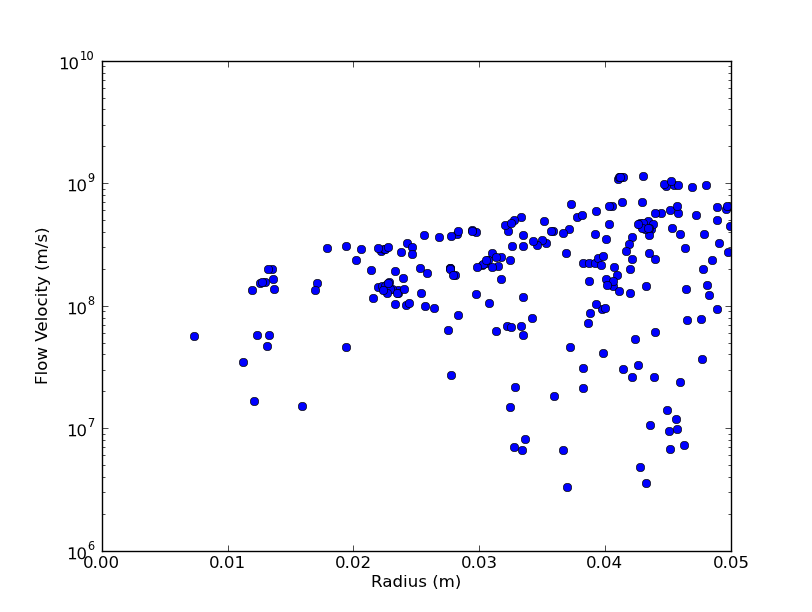
\includegraphics[width=5in, clip=true, trim=0in 0in 0.5in 0.5in]{../images/cylinder_velocity_profile.png}
\caption{Turbulent velocity in cylinder test case}
\end{figure}

\begin{figure}[H]
\centering
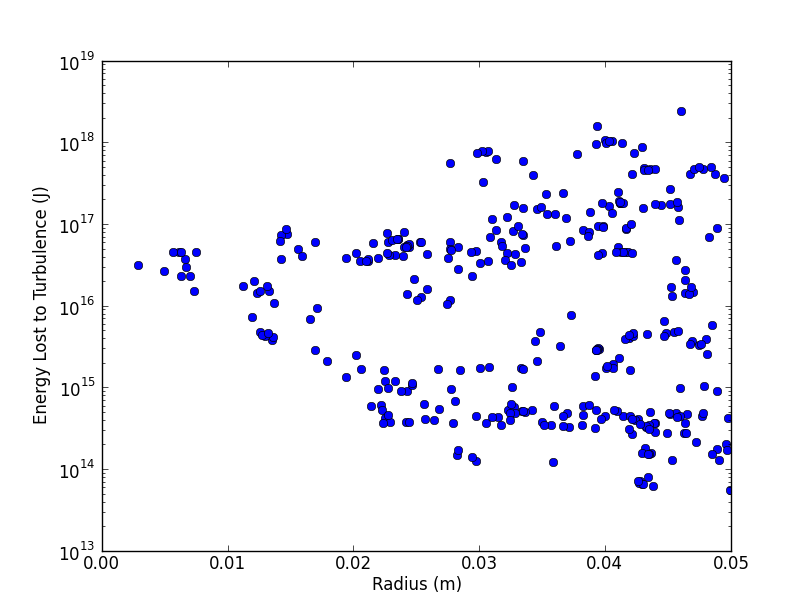
\includegraphics[width=5in, clip=true, trim=0in 0in 0.5in 0.5in]{../images/cylinder_turb_profile.png}
\caption{Turbulent energy in cylinder test case}
\end{figure}

The leading edge of the cylinder was normal to the fluid velocity, and this 
was likely the source of this problem.  The $k-\epsilon$ model fails in
cases with large pressure gradients, and the flow colliding with this
surface may have caused the turbulence model to produce unphysical turbulent
kinetic energies.

This problem could likely be corrected by replacing the flat surfaces with 
rounded ones, or using a more robust turbulence model.

\section{Conclusion}
The data I obtained in this project is not as conclusive as I would have hoped.
While it appears that the NACA5420 is actually excellent for laminarizing the
airflow in my duct, a certainly useful property, none of my airfoils produced
a statistically significant increase in mean velocity through the duct.  This
isn't very surprising, since I didn't actually simulate an airfoil 
around a fan, but an airfoil placed in front of a fan, and ducts placed around
fans are usually there to improve fan performance.

I really only was able
to scratch the surface of the many problems involved in simulating fluid flow, 
and a larger, future project could go in many directions.  I would have liked to
examine in more depth the turbulence modelling, perhaps by looking at other
models than $k-\epsilon$, as well as actually iterating through designs to
improve the performance, rather than just comparing a random selection of 
airfoils.  With numerical tools for analyzing flow, design work such as this
has become extremely efficient, and the entire parameter space of the NACA
airfoils could easily be probed with only a few months of CPU time.  Along with
tools like CNC machining, entire designs can move from idea to physical 
product using nothing more than a computer.

\section*{References}
\begin{enumerate}
\item \textit{Aerospace Globalization 2.0: Implications for Canada's Aerospace
Industry} AeroStrategy Management Consulting, November 2009

\item \textit{Code\_Saturne User Manual} EDF R\&D, December 2011 
(retrieved from\\ 
\verb!http://research.edf.com/fichiers/fckeditor/Commun/Innovation/!\\
\verb!logiciels/code_saturne/Documents/2.1/user.pdf!)

\item \textit{Code\_Saturne Theory Manual} EDF R\&D, December 2011
(retrieved from\\
\verb!http://research.edf.com/fichiers/fckeditor/Commun/Innovation/!\\
\verb!logiciels/code_saturne/Documents/2.1/theory.pdf!)
\item \textit{Aerodynamics of Wind Turbines} Martin O. L. Hansen, Routledge
December 2007

\item \textit{Code\_Saturne: a Finite Volume Code for the Computation of
Turbulent Incompressible Flows - Industrial Applications} Fr\'{e}d\'{e}ric
Archambeau, Namane M\'{e}chitoua, \& Marc Sakiz, International Journal on Finite
Volumes, Vol 1, 2004

\item \textit{The Characteristics of 78 Related Airfoil Sections From Tests In
The Variable Density Wind Tunnel} E. N. Jacobs, K. E. Ward, \& R. M. Pinkerton,
NACA Report No. 460, 1933
\end{enumerate}

\section*{Software Used}
\begin{itemize}
\item OpenSCAD  \textit{www.openscad.org}
\item Fully parametric NACA 4 digit Airfoil/Wing profile 
\textit{http://www.thingiverse.com/thing:10513}
\item gmsh \textit{geuz.org/gmsh/}
\item Code\_Saturne \textit{www.code-saturne.org}
\item paraView \textit{www.paraview.org}
\item Python \textit{www.python.org}
\item Numpy \textit{www.numpy.scipy.org}
\item Matplotlib \textit{matplotlib.sourceforge.net}
\end{itemize}
\end{document}
